% 
% Annual Cognitive Science Conference
% Sample LaTeX Paper -- Proceedings Format
% 

% Original : Ashwin Ram (ashwin@cc.gatech.edu)       04/01/1994
% Modified : Johanna Moore (jmoore@cs.pitt.edu)      03/17/1995
% Modified : David Noelle (noelle@ucsd.edu)          03/15/1996
% Modified : Pat Langley (langley@cs.stanford.edu)   01/26/1997
% Latex2e corrections by Ramin Charles Nakisa        01/28/1997 
% Modified : Tina Eliassi-Rad (eliassi@cs.wisc.edu)  01/31/1998
% Modified : Trisha Yannuzzi (trisha@ircs.upenn.edu) 12/28/1999 (in process)
% Modified : Mary Ellen Foster (M.E.Foster@ed.ac.uk) 12/11/2000
% Modified : Ken Forbus                              01/23/2004
% Modified : Eli M. Silk (esilk@pitt.edu)            05/24/2005
% Modified : Niels Taatgen (taatgen@cmu.edu)         10/24/2006
% Modified : David Noelle (dnoelle@ucmerced.edu)     11/19/2014

%% Change "letterpaper" in the following line to "a4paper" if you must.

\documentclass[10pt,letterpaper]{article}

\usepackage{cogsci}
\usepackage{pslatex}
\usepackage{apacite}

% our packages
% ---------------------------------------------------------
% \usepackage{hyperref}       % hyperlinks
% \usepackage{url}            % simple URL typesetting
\usepackage{subcaption}
\usepackage{amsmath,amsfonts,amsthm,amssymb,amsopn,bm}
\newcommand{\vct}[1]{\boldsymbol{#1}} % vector
\newcommand{\mat}[1]{\boldsymbol{#1}} % matrix

\usepackage{graphicx}
\graphicspath{{../graphs/}}
% ----------------------------------------------------------


\title{Selecting Between Competing Computational Models of the Stroop Task \\ On the Bases of Effective Connectivity}
 
\author{{\large \bf Micah Ketola (ketolm@uw.edu)} \\
  Department of Psychology, Campus Box 351525, \\
  Seattle, WA 98195 USA
  \AND {\large \bf Linxing Preston Jiang (prestonj@cs.washington.edu)} \\
  Paul G. Allen School of Computer Science and Engineering\\
  Seattle, WA 98195 USA 
  \AND {\large \bf Andrea Stocco (stocco@uw.edu)} \\
  Department of Psychology and Institute for Learning and Brain Sciences (I-LABS), Campus Box 351525, \\
  Seattle, WA 98195 USA}


\begin{document}

\maketitle


\begin{abstract}
Recent advances have made it possible to generate fMRI predictions for cognitive architectures, such as ACT-R, thus expanding on the possible data to be explained and making it possible to distinguish models between alternative models that make otherwise identical behavioral predictions. However, for tasks associated with relatively brief response times, fMRI predictions are often not sufficient to provide adequate identifiability. In this paper, we outline a method based on {\it effective connectivity}, which significantly augments the amount of information that can be extracted from fMRI data to distinguish between model. We show the application of this method in the case of two competing ACT-R models of the Stroop task. Although the models make, predictably, identical behavioral and BOLD time-course predictions, patterns of functional connectivity favor on model over the other. Finally, we show that the same data suggests directions in which both models should be revised.

\textbf{Keywords:} 
ACT-R, Dynamic Causal Modeling, Cognitive Science
\end{abstract}

\section{Introduction}

One of the traditional problems in the field of cognitive modeling is deciding which of two models is right. The most common procedure to compare two models is to use null- hypothesis testing procedures. In essence, conditions are identified in which the two models make qualitatively different predictions, and the hypothesized pattern is tested using classical techniques. While more sophisticated approaches have been proposed \cite{Pitt2006, Veksler2015}, this approach remains the {\it de facto} standard of the field.

The search for conditions in which two models differ is sometimes streneous. The same behavior can sometimes be obtained through different possible internal processes and mdoel parameters. By shedding light on more direct correlates of cognitve processes, neuroimaging data provides a potential way to distinguish between otherwise behaviorally identical results \cite{Sohn2004}. For this reason, procedures have been devised to draw neuroimaging predictions from computational models, most commonly using fMRI (\cite{Anderson2008}).

While the use of fMRI has greatly expanded upon the possible predictons that can distinguish between the two models, a number of limitations still exist. The major limitation is due to the limited temporal resolution of fMRI. 
However, even methods that offer a more precise temporal resolution, such as EEG or MEG, suffer from drawbacks. For example, models often rely on specific, crucial assumptions about the order of mental steps of the causal relationship between different modules. 

Recently, Rice and Stocco (2019) proposed using TMS as a different way to test model predictions. TMS provides a way to causally interfere with specific cortical computations, thus providing both causal interference and the necessary spatio-temporal resolution. It should be noted, however, that their paper did not use this technique to compare models. 

In this paper, we describe and demonstrate an alternative and novel way to test models using neuroimaging data that addresses these concerns. This method is based on patterns of {\it effective connectivity} between brain regions. Effective connectivity is an umbrella term to characterize the functional exchange of information between two brain regions, based on the analysis of their respective time series. Because effective connectivity provides measures of directional communication between two regions, it can be used to examine the internal dynamics of a computational model.  Furthermore, because effective connectivity can be estimated from fMRI or EEG data, it expands the dimensions across which models can be compared without requiring collecting additional data.

In the reminder of this paper, we will outline our method and apply it to a specific, and exquisitely cognitive, case, namely, determining which of two prominent computational explanations for the Stroop interference best explains the data.    

\subsection{ACT-R}

Although our method could be applied to any computational model, for convenience, it will be demonstrated with two models developed in the Adaptive Control of Thought--Rational (ACT-R) cognitive architecture \cite{Anderson2004}. This choice was made for three reasons.  First, ACT-R is the most successful and widespread architecture, having been used in hundreds of publications since its inception, and by far the most popular in the field of cognitive research \cite{Kotseruba2018}; Thus, it provides an excellent domain in which to demonstrate the procedure.

Second, ACT-R already provides well-tested mappings between architectural components and brain regions and established procedures to predict fMRI activity from model simulations. Therefore, these assumptions can be adopted without the need to provide additional justifications.

Finally, the assumptions of ACT-R provide reasonable mechanism to translate model activity into effective connectivity. As it will be shown, this is based on the functional requirements of the procedural module, which have been examined and discussed in the past.

Fig. 1 provides an overview of the ACT-R architecture and introduces the graphical conventions that will be used in other figures of this paper to indicate different architectural components. Consistent with current views in neuroscience, ACT-R stores knowledge in two formats, declarative and procedural. Declarative knowledge is stored in vector-like structures called chunks, which are used to represent static information like semantic memories (“Paris is the capital of France”), perceptual inputs (“A black triangle is on the screen”), or motor commands (“Press the spacebar”). In Fig. 1, chunks are represented by the flowchart symbol of a document. Procedural knowledge, on the other hand, consists of production rules (or simply “productions”), state-action associations that encode basic operations and procedures as well as the specific knowledge to perform the various steps of a task. In Fig. 1, productions are represented with the flowchart symbol of a process (a square), with incoming arrows representing the state in which the action is applied (also known as ``condition'') and outgoing arrows representing their action. Thus, chunks represent information, and productions act upon them.

The relationship between chunks and productions is mediated by a set of functional modules (solid rounded rectangles in Fig. 1). For instance, perceptual modules create new chunks to represent the contents of the outside world, and a memory module maintains chunks in long-term memory. Chunks are made available to production rules via a set of module-specific buffers, (dashed rounded rectangles in Fig. 1). Only when chunks are placed into buffers, can they be inspected, modified, and copied by production rules. 

As noted above, much work has been dedicated to map ACT-R modules to corresponding neural circuits (Anderson, 2007; Anderson, Albert, & Fincham, 2005; Anderson et al., 2008; Borst et al., 2010; Fincham & Anderson, 2006; Fincham, Carter, Van Veen, Stenger, & Anderson, 2002; Stocco & Anderson, 2008). This work has yielded a number of reliable functional mappings, including the association between anterior cingulate cortex and the goal buffer in the goal module (Fincham & Anderson, 2006; Sohn, Albert, Jung, Carter, & Anderson, 2007), between the lateral prefrontal cortex and the retrieval buffer of the long-term memory module (Anderson, 2005; Danker, Gunn, & Anderson, 2008; Fincham & Anderson, 2006), between posterior parietal cortex and the imaginal buffer of working memory (Anderson, 2005; Anderson, Albert, et al., 2005; Borst et al., 2010; Sohn, Ursu, Anderson, Stenger, & Carter, 2000), between the fusiform gyrus and the visual buffer in the visual module (Anderson, 2005; 2007), and between the primary motor cortex and the manual buffer in the motor module (Anderson, 2005; Anderson et al., 2004).

For the purpose of this paper, the most relevant mapping is the one between the procedural module and the basal ganglia (Anderson, 2005; Anderson et al., 2008; Stocco & Anderson, 2008). In addition to the fact that the activity trace of the procedural module predicts the BOLD response in the basal ganglia (Anderson, 2005; Anderson et al., 2008; Stocco & Anderson, 2008), this identification relies on a number of other arguments

\subsection{Dynamic Causal Modeling}

To estimate effective connectity, we adopted a framework known as Dynamic Causal Modeling (DCM) \cite{Friston2003, Stocco2018}. In essence, DCM is procedure to model the time-course of in brain activity in a set of brain regions through a dynamical system of other brain regions and event vectors. Specifically, the time course of activity of a region $i$ is expressed as a bilinear state equation:

\[\dot{\vct{y}} = \mat{A}\vct{y} + \sum_{i}x_i\mat{B}(i)\vct{y} + \mat{C}\vct{x}\]

where $\mat{A}$ defines intrinsic connectivity between different regions (fixed connectivity), $\mat{C}$ defines effects by task inputs, and $\mat{B}$ defines the modular effects that task conditions have on the connectivity between regions (modulation of connectivity). The overall ``effect'' of one module to another was then approximated by the element-wise product of $\mat{A}$ and $\mat{B}$, namely
\[\text{effective connectivity} = \mat{A} \odot \mat{B}\]

\subsection{Deriving ACT-R Predictions for Effective Connectivity }

Since each trial the Stroop task is generally performed within one second, it is expected that the three information processing modules: imaginal, goal, and retrieval should have strong correlations since their activation could only be captured in one image scan given our sampling rate $TR = 1.5$ seconds. Furthermore, if the imaginal module is for intermediate information processing as ACT-R suggests, an increasing connectivity effect from imaginal module to goal module ("problem state") is expected in order to process the unmatching color and text semantics in incongruent trials.

\section{An Application of the Method: ACT-R Models of the Stroop Task}

To demonstrate this method, two models of the Stroop task were implemented. They were derived from previously proposed alternative models of the Stroop task, authored by Marsha Lovett \cite{Lovett2005} and by Erik Altmann \cite{VanMaanen2009}. Since both models were published before ACT-R underwent significant revisions, the two models were re-implemented in the most recent version of ACT-R (version 7.6). This reimplementation processes also ensured that the two models interacted with the task using the same sensorimotor mechanisms, i.e. visual objects and responses were given in the same way. From now on, we will refer to these two models as the Lovett-like model and the Altmann-like model. 

Despite the re-implementation, the two models maintained the underlying assumptions that underlied their original proposal. Specifically, the two models provide different explanations about the nature of Stroop interference. In the Lovett model, Stroop interference is driven by the tendency of the model to automatically process the word dimension of the stimulus first. In processing this dimension, \textit{word-association chunks}, linking words to their conceptual representation, are added to the imaginal buffer. From there, a response matching the representation is retrieved and the model then either responds using this representation, or checks if the representation matches the visual color seen. If there is not a match, then the color dimension of the stimulus is processed and \textit{color-association chunks} are added to the imaginal buffer, linking colors to their conceptual representations. 

%Traditionally, hemodynamic response functions (HRFs) are convolved with the event matrix (i.e., information processing of each module) derived from ACT-R to simulate fMRI data for various tasks \cite{Anderson2004,Lindquist2009}. A common choice of HRF, the double gamma function, is define as 
%\[f(t, \alpha, \beta) = \frac{t^{\alpha - 1}e^{-\beta t}}{\Gamma(\alpha)}\]
%where $t$ is time, $\alpha$ and $\beta$ define the scale and shape of the function, respectively, and $\Gamma(x) = (x - 1)!$ for $x \in \mathbf{R}$ \cite{Poldrack, Cignetti2016}. Then the simulated data is visually compared to the real fMRI data to check for similarities, or simple metrics such as mean square error are applied \cite{Anderson2004, Borst2017}. More rigorous analysis without the assumption of brain activations being HRF-shaped could be useful to verify ACT-R in a bottom-up approach. In this project, both brain connectivity analysis and mixture models are proposed to discover meaningful structures directly from the data with few assumptions. Specifically, covariance estimation and dynamic causal modeling were used to study brain region connectivity, and Gaussian Mixture Models were used to estimate the distributions of individual brain activation in each module.

\section{Materials and Methods}

\subsection{Experimental Dataset}

In this analysis, we used fMRI publicly available from on an open repository\footnote{The data is available on OpenNeuro at the following URL:  https://openneuro.org/datasets/ds000164/versions/00001}. The original data was collected at Carnegie Mellon University by Timothy Verstynen, and published in Verstynen et al. \cite{Verstynen2014}.

\subsection{Participants}

\subsection{Experimental Task}

The data was collected while the subjects performed the Stroop task \cite{Stroop1935}, during which the subjects were asked to select the box whose color matched that of the text, however, the color of the text itself may (congruent trials) or may not (incongruent trials) match its semantic meaning. If, for example, the word "red" is shown on the screen painted in blue, then the subject is supposed to select the blue box instead of the red box.




\begin{figure}[ht]
\centering
  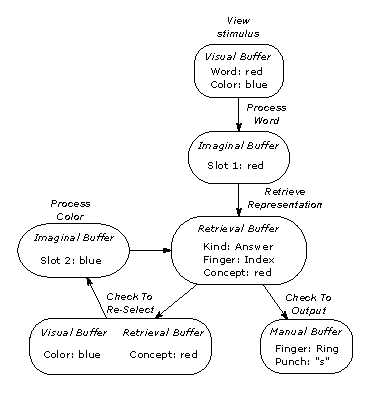
\includegraphics[width=\linewidth]{meaning_color_model.eps}
  \caption{This is my first model}
\end{figure}%

\begin{figure}[ht]
\centering
  
\includegraphics[width=\linewidth]{overall_model.eps}
  \caption{This is my second model}
\end{figure}%


\section{Data and Modeling}

The Talairach coordinates used for each module in the brain followed the convention used by \cite{Anderson2008, Borst2017}. The algorithms described in \cite{Lacadie2008} were used to convert Talairach coordinates to Montreal Neurological Imaging Institute (MNI) coordinates (see Appendix D). The region of interest (ROI) mask files were created through FSL \cite{Woolrich2009} of size 16 mm (125 voxels in total) then used to extract fMRI data from each ROI. The real fMRI data were head-motion corrected and smoothed by a 8-mm Gaussian kernel using SPM \cite{Penny2006}. Principle component analysis was then applied on the extracted fMRI data in each ROI. The largest principle component was used to project the original data to the new space with more than 75\% of the variance explained in each module.



\section{Result}

Figure~\ref{fig:conn} shows the connectivity analysis results between modules. Figure~\ref{fig:conn} (a) shows the functional connectivity between retrieval and imaginal is high as expected, while that between imaginal and goal is not as high. (b) and (c) show the results of DCM in both congruent and incongruent trials averaged across subjects through Bayesian parameter averaging \cite{Kasess2010} (see Appendix C), and (d) shows the difference in the effective connectivity in different tasks (incongruent - congruent). Circled parts in (d) confirm the effect we expect from ACT-R: in incongruent trials, there is a significant increase between imaginal and goal modules to account for the unmatching color and semantic condition. More importantly, their effect on the output (i.e., the manual module) also changes drastically. Compared to congruent trials, there is a significant decrease effect from goal to manual and a significant increase effect from imaginal to manual, suggesting that information about the final decision is delivered by imaginal rathar than goal in incongruent trials. Again, this supports ACT-R's assumption that little imaginal involvement is needed in congruent trials. 



\section{Formalities, Footnotes, and Floats}

Use standard APA citation format. Citations within the text should
include the author's last name and year. If the authors' names are
included in the sentence, place only the year in parentheses, as in
\citeA{NewellSimon1972a}, but otherwise place the entire reference in
parentheses with the authors and year separated by a comma
\cite{NewellSimon1972a}. List multiple references alphabetically and
separate them by semicolons
\cite{ChalnickBillman1988a,NewellSimon1972a}. Use the
``et~al.'' construction only after listing all the authors to a
publication in an earlier reference and for citations with four or
more authors.


\subsection{Footnotes}

Indicate footnotes with a number\footnote{Sample of the first
footnote.} in the text. Place the footnotes in 9~point type at the
bottom of the column on which they appear. Precede the footnote block
with a horizontal rule.\footnote{Sample of the second footnote.}


\subsection{Tables}

Number tables consecutively. Place the table number and title (in
10~point) above the table with one line space above the caption and
one line space below it, as in Table~\ref{sample-table}. You may float
tables to the top or bottom of a column, or set wide tables across
both columns.

\begin{table}[!ht]
\begin{center} 
\caption{Sample table title.} 
\label{sample-table} 
\vskip 0.12in
\begin{tabular}{ll} 
\hline
Error type    &  Example \\
\hline
Take smaller        &   63 - 44 = 21 \\
Always borrow~~~~   &   96 - 42 = 34 \\
0 - N = N           &   70 - 47 = 37 \\
0 - N = 0           &   70 - 47 = 30 \\
\hline
\end{tabular} 
\end{center} 
\end{table}


\subsection{Figures}

All artwork must be very dark for purposes of reproduction and should
not be hand drawn. Number figures sequentially, placing the figure
number and caption, in 10~point, after the figure with one line space
above the caption and one line space below it, as in
Figure~\ref{sample-figure}. If necessary, leave extra white space at
the bottom of the page to avoid splitting the figure and figure
caption. You may float figures to the top or bottom of a column, or
set wide figures across both columns.

\begin{figure}[ht]
\centering
\begin{subfigure}{.5\textwidth}
  \centering
  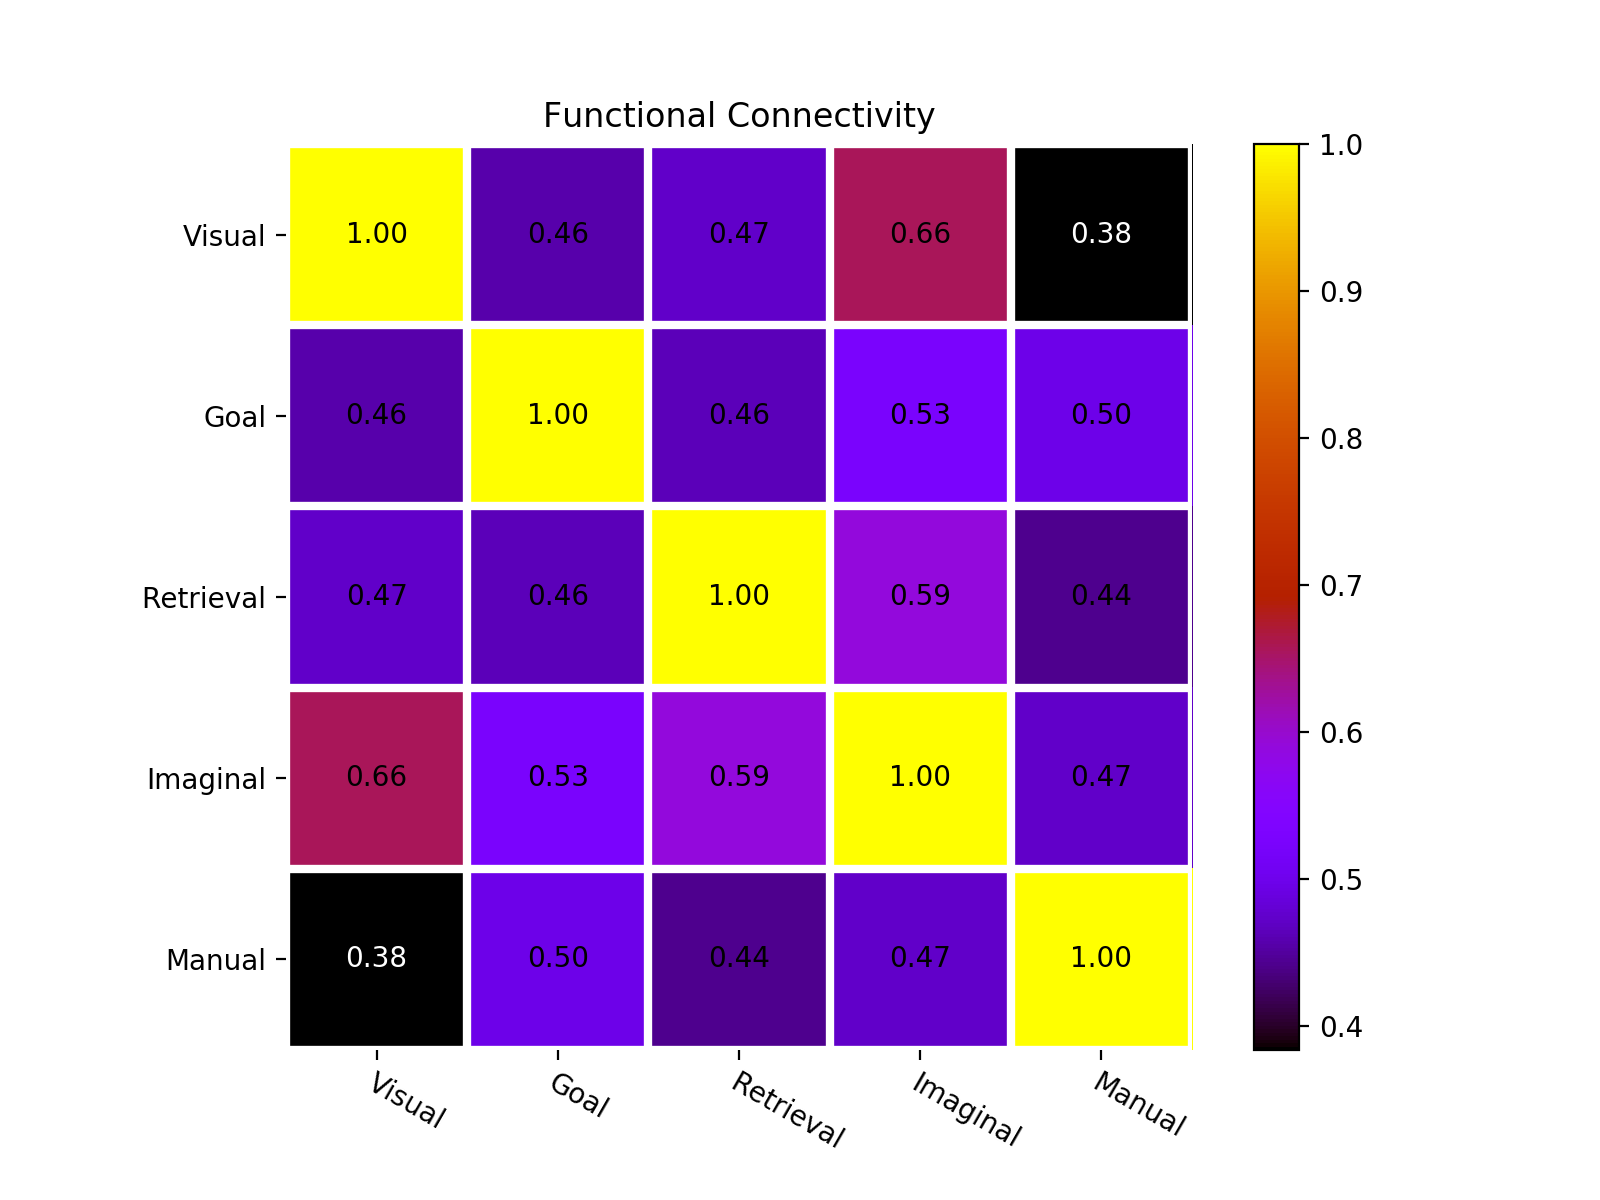
\includegraphics[width=\linewidth]{func_conn.png}
  \caption{}
\end{subfigure}%
\begin{subfigure}{.5\textwidth}
  \centering
  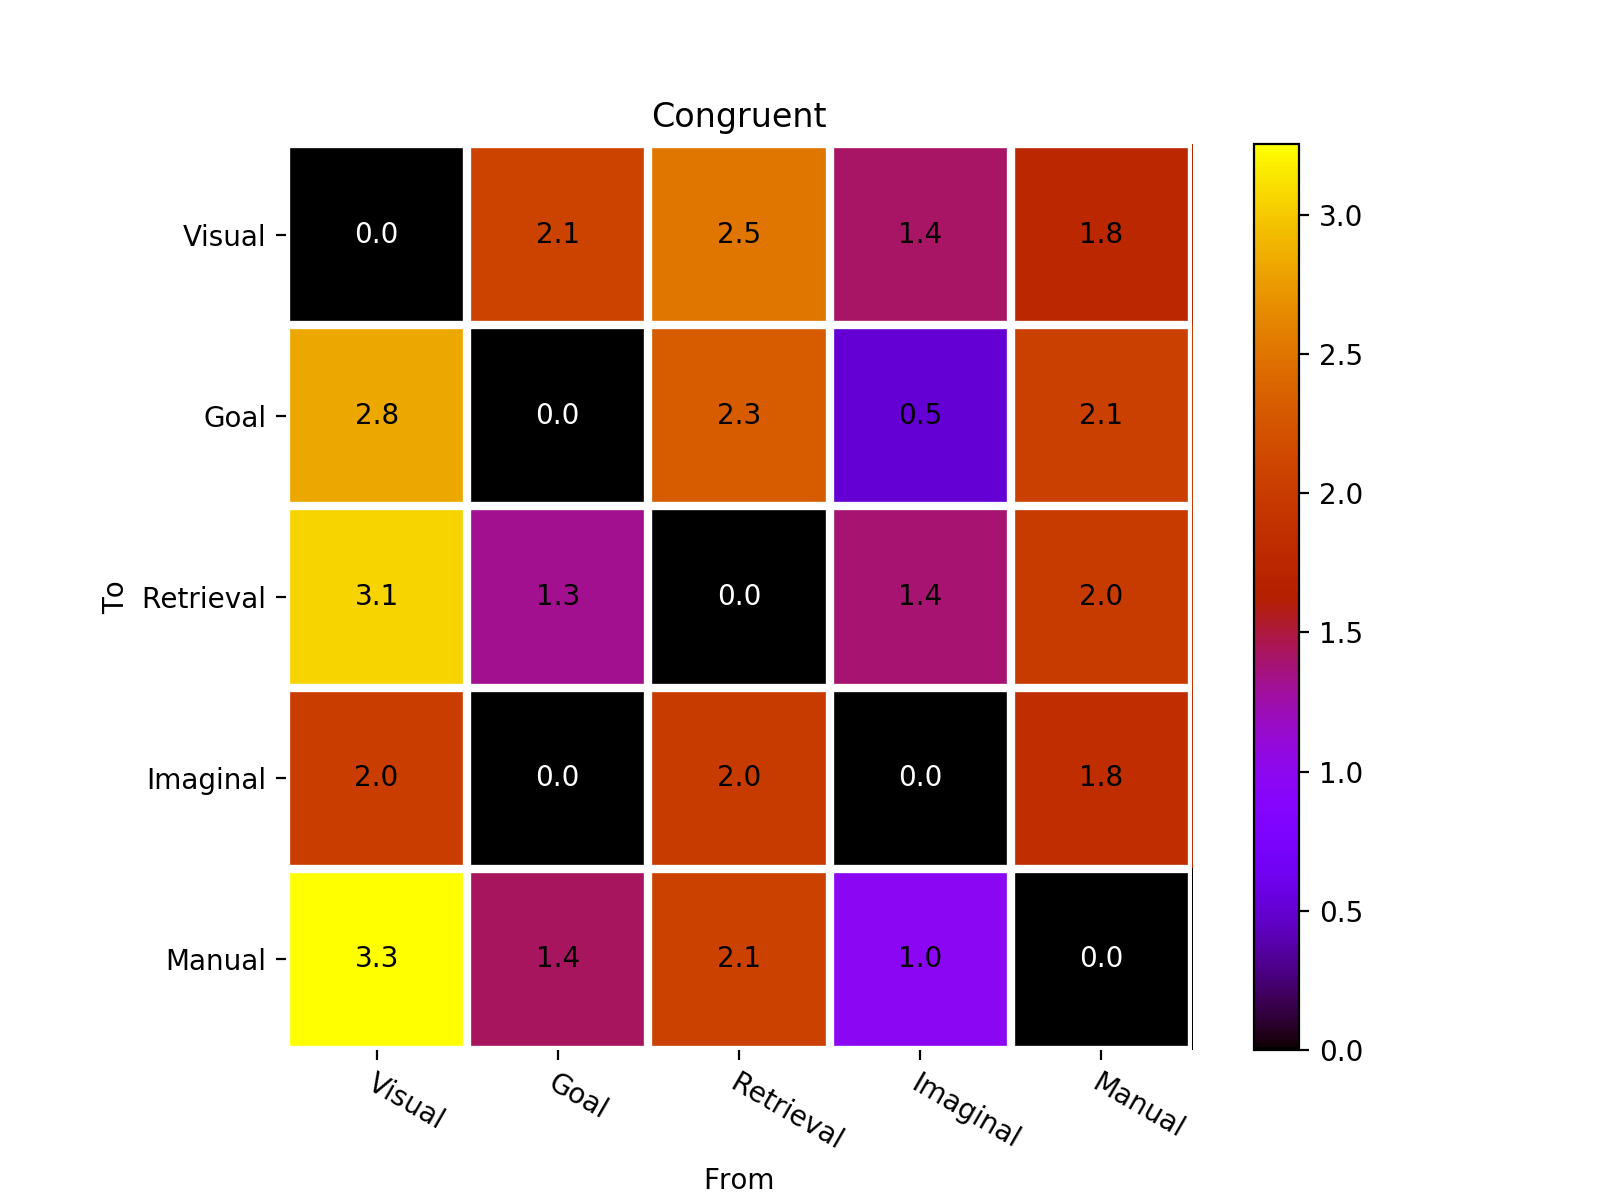
\includegraphics[width=\linewidth]{Congruent_effect_conn.png}
  \caption{}
\end{subfigure}
\begin{subfigure}{.5\textwidth}
  \centering
  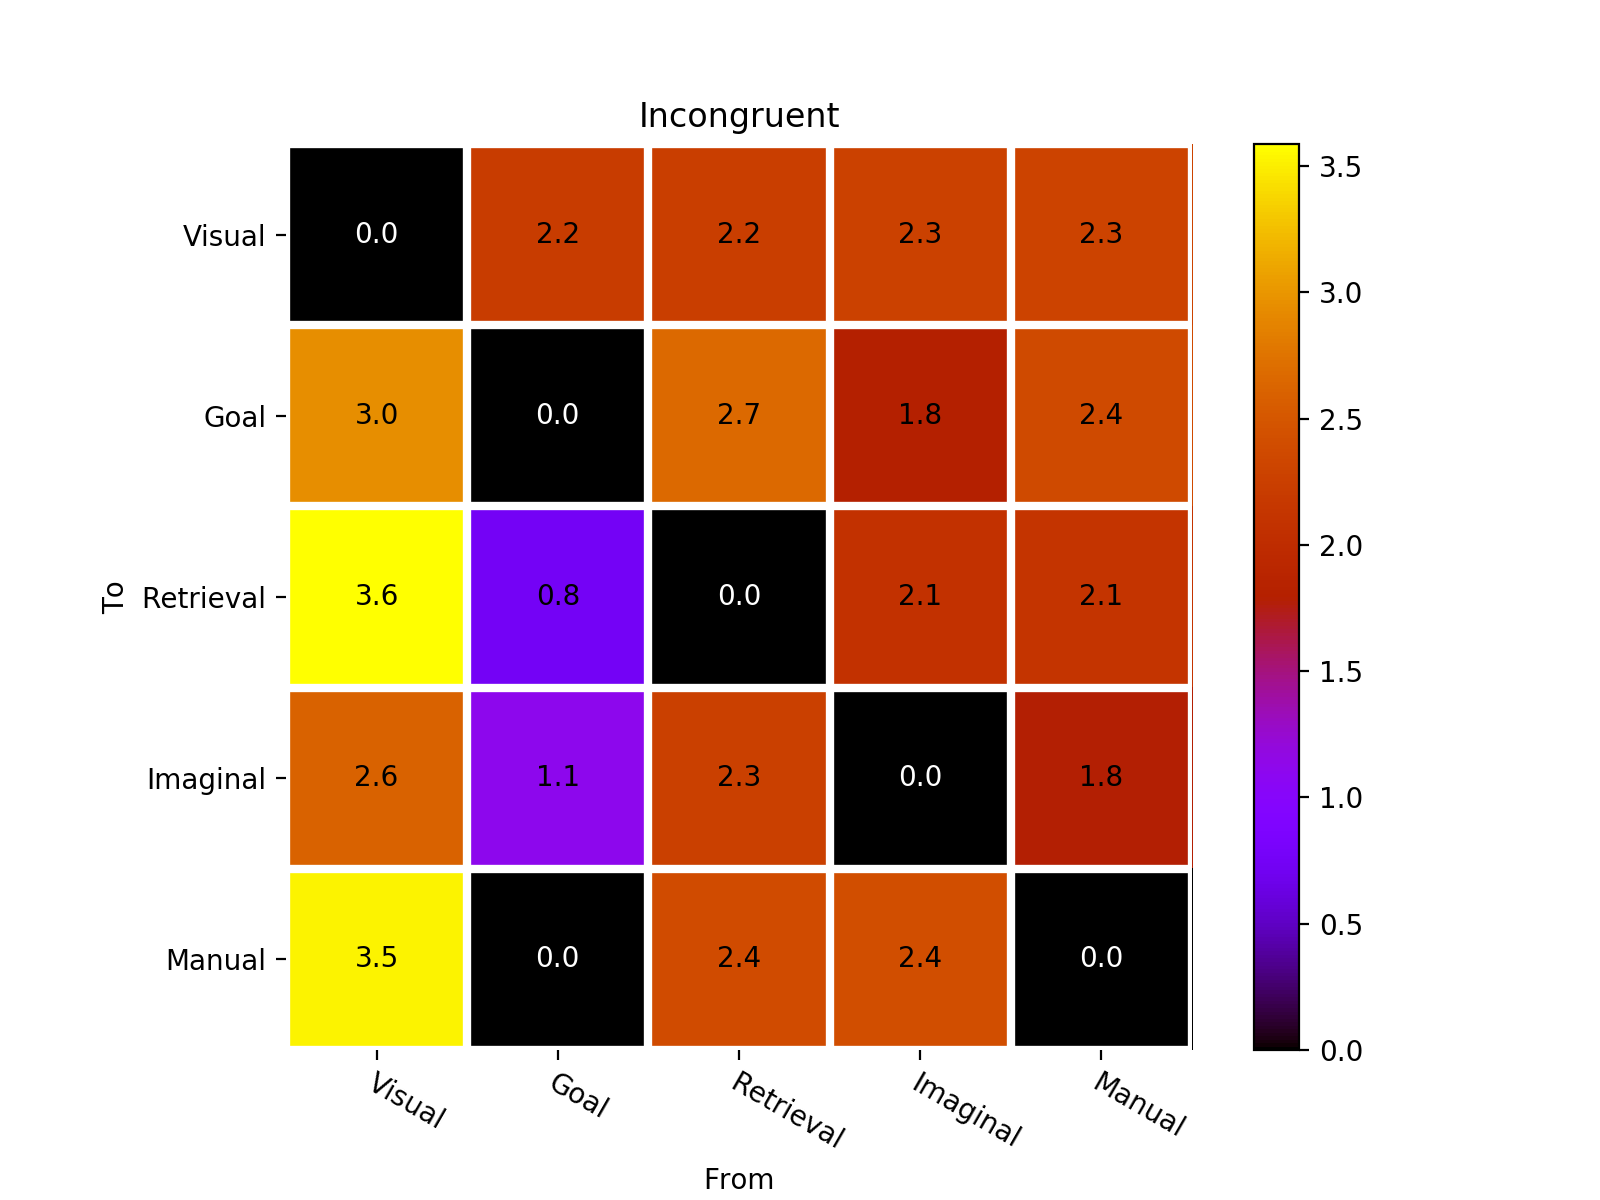
\includegraphics[width=\linewidth]{Incongruent_effect_conn.png}
  \caption{}
\end{subfigure}%
\begin{subfigure}{.5\textwidth}
  \centering
  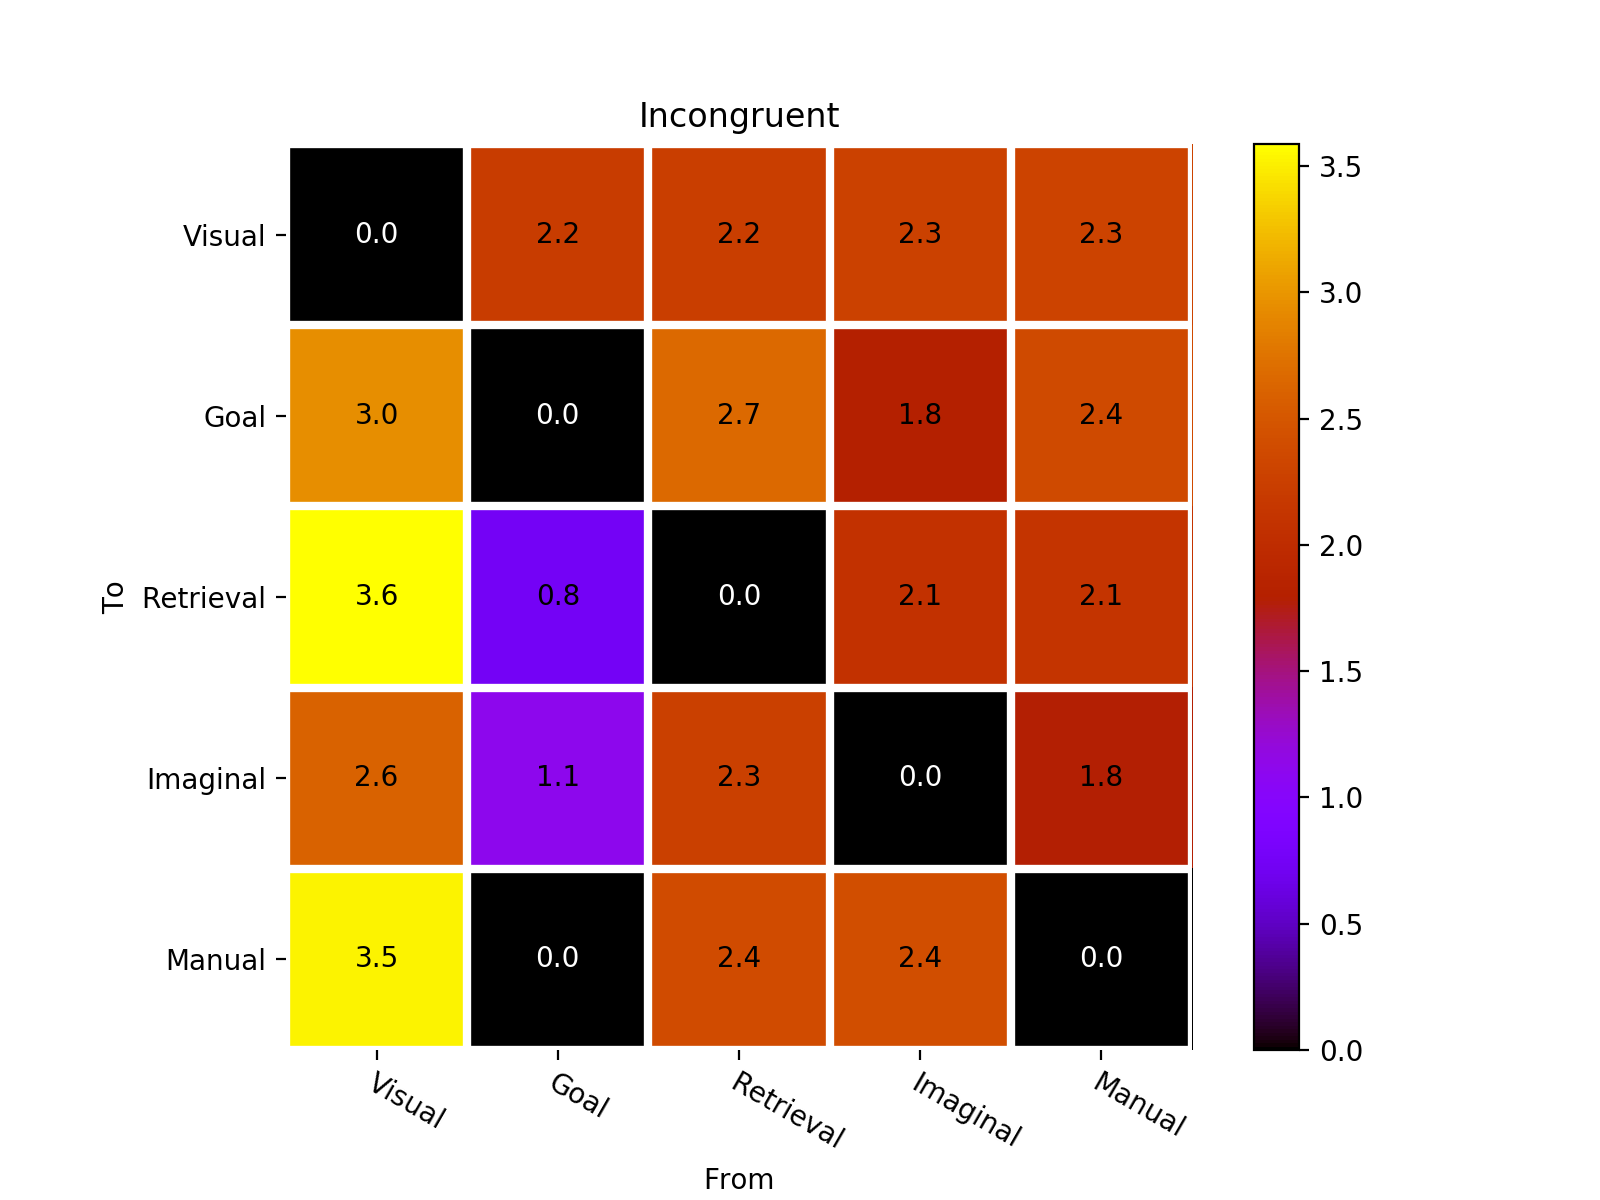
\includegraphics[width=\linewidth]{Incongruent_effect_conn.png}
  \caption{}
\end{subfigure}
\caption{Brain region connectivity results: (a) Functional connectivity analysis shows strong brain signal activation between imaginal and retrieval, but not imaginal and goal; (b) Effective connectivity in congruent trials: similar strong effects between retrieval and imaginal are shown (data is zero-min) ; (c) Effective connectivity in incongruent trials: increasing connectivity between imaginal and goal are shown (data is zero-min); (d) Difference of effective connectivity in different tasks (incongruent - congruent): circled regions show brain connectivity dynamics in different tasks.}
\label{fig:conn}
\end{figure}


\begin{figure}[ht]
\begin{center}
\fbox{CoGNiTiVe ScIeNcE}
\end{center}
\caption{This is a figure.} 
\label{sample-figure}
\end{figure}


\section{Acknowledgments}

Place acknowledgments (including funding information) in a section at
the end of the paper.


\section{References Instructions}

Follow the APA Publication Manual for citation format, both within the
text and in the reference list, with the following exceptions: (a) do
not cite the page numbers of any book, including chapters in edited
volumes; (b) use the same format for unpublished references as for
published ones. Alphabetize references by the surnames of the authors,
with single author entries preceding multiple author entries. Order
references by the same authors by the year of publication, with the
earliest first.

Use a first level section heading, ``{\bf References}'', as shown
below. Use a hanging indent style, with the first line of the
reference flush against the left margin and subsequent lines indented
by 1/8~inch. Below are example references for a conference paper, book
chapter, journal article, dissertation, book, technical report, and
edited volume, respectively.

\bibliographystyle{apacite}
\setlength{\bibleftmargin}{.125in}
\setlength{\bibindent}{-\bibleftmargin}
\bibliography{ref}


\end{document}
